\documentclass[12pt]{article}

%%%%%%%%%%%%%%%%%%%%%%%%%%%%%%%%%%%%%%%%%%%%%%%%%%%%%%%%%%%%%%%%%%%%%%
%% This section is called the preamble, where we can specify which
%% latex packages we required.  Most (but not of all) of the packages
%% below should be fairly standard in most latex documents.  The
%% exception is xspace and the new \latex command, which you probably
%% do not need.
%%%%%%%%%%%%%%%%%%%%%%%%%%%%%%%%%%%%%%%%%%%%%%%%%%%%%%%%%%%%%%%%%%%%%%

%% Better math support:
\usepackage{amsmath}
\usepackage{algorithm,algpseudocode}
%\usepackage{algorithm}
%\usepackage{algorithmic}
%\usepackage{algorithmicx}
%\usepackage{algorithm2e}
%\usepackage[noend]{algpseudocode}
%\usepackage{breqn}

%% Bibliography style:
\usepackage{mathptmx}           % Use the Times font.
\usepackage{graphicx}           % Needed for including graphics.
\usepackage{url}                % Facility for activating URLs.

%% Set the paper size to be A4, with a 2cm margin
%% all around the page.
\usepackage[a4paper,margin=3cm]{geometry}

%% Natbib is a popular style for formatting references.
% %\usepackage{bib}

%\usepackage{subcaption}
\usepackage{subfig}

\usepackage{pdflscape}

\usepackage{placeins}

\usepackage{natbib}
% %\usepackage[abbr]{harvard}
%% bibpunct sets the punctuation used for formatting citations.
\bibpunct{(}{)}{;}{a}{}{,}

%% textcomp provides extra control sequences for accessing text symbols:
\usepackage{textcomp}
\newcommand*{\micro}{\textmu}
%% Here, we define the \micro command to print a text "mu".
%% "\newcommand" returns an error if "\micro" is already defined.

\usepackage{setspace}

%% This is an example of a new macro that I've created to save me
%% having to type \LaTeX each time.  The xspace command provides space
%% after the word LaTeX where appropriate.
\usepackage{xspace}
\providecommand*{\latex}{\LaTeX\xspace}
%% "\providecommand" does nothing if "\latex" is already defined.

\usepackage{titling}
\newcommand{\subtitle}[1]{%
  \posttitle{%
    \par\end{center}
    \begin{center}\large#1\end{center}
    \vskip0.5em}%
}

\makeatletter
\def\BState{\State\hskip-\ALG@thistlm}
\makeatother

%%%%%%%%%%%%%%%%%%%%%%%%%%%%%%%%%%%%%%%%%%%%%%%%%%%%%%%%%%%%%%%%%%%%%%
%% Start of the document.
%%%%%%%%%%%%%%%%%%%%%%%%%%%%%%%%%%%%%%%%%%%%%%%%%%%%%%%%%%%%%%%%%%%%%%

\begin{document}

\author{Markus Neumann\\
  The Pennsylvania State University}
\date{\today}
\title{\textbf{One for all and all for one?}}
\subtitle{Altruistic behavior, population size and network topology}
\maketitle

\doublespacing
\begin{abstract}
The question of why acts of selflessness occur in a Hobbesian self-help world has fascinated scholars for decades, if not centuries. Utilizing simulations, previous research has shown that altruism can be evolutionarily stable in small-scale societies under a narrow set of circumstances. However, when expanding such models to populations of anything larger than a few hundred people, they generally break down. In this paper, I modify the widely used image-score mechanism to include contagion-based reputation and demonstrate how altruism can survive in populations of up to 20,000. I also find that selflessness strongly depends on network topology - with important implications for issues such as social capital and the structure of political organizations.
\end{abstract}

\section*{Introduction}
Altruism is a great behavioral puzzle. People help the homeless, donate blood, or give to charity - with no discernible reward for themselves. In spite of the many incentives to defect, humans choose to cooperate with one another on a daily basis. The progression of evolutionary research on this phenomenon can be characterized as a path from small- to large-N explanatory power:

`Inclusive fitness' provides an explanation for altruism between family members \citep{Hamilton1964}. In order to pass on its genes, an organism's best chance is to reproduce, and failing that, to aid its closest relatives in doing so. However, Hamilton's theory does not account for altruism outside the family.

Indirect reciprocity fills this role by adding reputation into the equation: I scratch your back, and while you don't necessarily have to scratch mine, my reputation built in the process will ensure my back will get scratched by someone. Using this approach, altruism has been shown to be evolutionarily stable in populations of up to 100 \citep{Nowak1998}. However, \cite{Nowak1998} also point out that as population size increases, establishing cooperation becomes much more difficult. Network approaches have since managed to raise this number to around 300, with \cite{Peleteiro2014} even reaching 1000. But eventually, altruism breaks down without fail. Evidently, the extant literature fails to account for selfless behavior in anything larger than a small village. Humans have congregated in much bigger cities for thousands of years, a trend that has only accelerated since the Industrial Revolution. Consequently there is a need to explain how altruism can exist in larger populations. In this paper, I take the next step in this line of research: Under which parameters is altruism evolutionarily stable in a population of up to 20,000?

The key to solving this problem has already been hinted at by the network reciprocity literature: Network topology, which translates to population density and clustering (i.e. neighborhoods), has been shown to have an effect on cooperative behavior \citep{Santos2008,Peleteiro2014}, but due to the common assumption of perfect information across the network, this has not yet been brought to its logical conclusion. I do so by first introducing a contagion mechanism through which information spreads throughout the network. Then, I compare random networks generated with the  Watts-Strogatz algorithm \citep{Watts1998}, which, depending on the model parameters, can produce a small-world network, with a number of neighborhoods within which players are very densely connected. Connections between the neighborhoods themselves however are much more sparse. As such, it realistically mimics social structures formed by humans, such as families, neighborhoods, or villages: people living within these structures are much more closely connected to other members of these structures and interact with them on a more frequent basis, but nevertheless maintain some level of contact with the outside world as well. This means that the small-world network alleviates the problem a large population poses to altruism, as it essentially consists of a number of smaller sub-populations, which are much more amenable to altruistic behavior.
%Building on \cite{Nowak1998}, I utilize the donation game, because it captures all important aspects of indirect reciprocity in a parsimonious manner: one person helps out another at his own detriment, but benefits in the form of an improved reputation. Therefore he is more likely to receive help from someone else in the future. I modify the image score mechanism for greater compatibility with networks, while staying as true to \cite{Nowak1998} as possible to ensure comparability with the extant literature.

% -- sign post
I begin by situating my analysis within the body of research on indirect and network reciprocity. Here, I also provide some context for how this research may be applied to phenomena such as social capital and political organizations. A new contagion-based method for handling image scores is introduced, designed to be more realistic and receptive to different network topologies. This leads to a set of novel results: altruistic behavior is demonstrated in populations of up to 20,000, and shown to be strongly dependent on the structure of the network. Substantively, this means that egalitarian groups and societies are at an advantage when it comes to encouraging selfless behavior among their members. Large-scale groups on the other hand face difficulties when it comes to fostering altruism. I show that given the right structure, this problem can however be ameliorated.

\section*{The Evolutionary Stability of Altruism}
%-- Kin Selection
Altruism between nonhuman animals can be explained through 'inclusive fitness'. Conceived by William \cite{Hamilton1964}, one of Darwin's most famous successors, this theory accounts for selflessness through the bonds of family: The parents, siblings and children of an organism have a 50 percent chance of sharing an allele for any one gene. In order to pass on its genes, an organism's best chance is to reproduce, and failing that, to aid its closest relatives in doing so. Ergo, costly altruistic behavior towards these individuals is rational because it increases their reproductive fitness.

A good showcase for this concept is provided by animals warning their relatives when sighting a predator. Examples include the ''thumping'' of rabbits, as well as warning cries by birds and monkeys \citep{hamilton1964_2}. The sentry reduces its own chances of survival, as it attracts the attention of the predator and spends time alerting its family rather than fleeing immediately. However, it also increases the reproductive fitness of its kin, and thus makes it more likely that its own genes will be passed on.

This concept is expressed in the simple equation $rB > C$. If the benefits $B$ of an altruistic action, controlling for the degree of relatedness $r$ (the probability of sharing any one gene), are greater than the costs $C$, said action is worth undertaking.

%-- Alternatives to kin selection
In principle, inclusive fitness also applies to humans. However, it does not have the same explanatory power as for other animals \citep{Abbot2013}. While altruistic behavior between unrelated nonhuman animals is extremely rare, it occurs frequently among \textit{homo sapiens} \citep{Axelrod1981,Fehr2002}. Evolutionary game theory offers several alternatives to kin selection: Direct reciprocity, group selection, altruistic punishment, indirect reciprocity and network reciprocity number among the most prominent ones.

%-- Direct reciprocity
Direct reciprocity frames cooperative behavior as a simple quid pro quo interaction: you scratch my back and I will scratch yours. This theory features strongly in the economist tradition and is useful for explaining a wide range of behaviors \citep{Axelrod1981,Fehr2002}. However, it falls short when dealing with sporadic encounters in large-scale societies, where it is unlikely that two individuals will meet twice. People are usually willing to help a stranger in need even if it is unlikely that this person will ever get the chance to reciprocate. More importantly, both parties receive an immediate benefit. As a result, true altruism, which would presuppose unconditional benevolence, is not present here \citep{Fehr2000}. Consequently I do not make use of this mechanism.

%-- Group Selection
The same is true for group selection. Originally conceived in the 1960s, this theory has been picked up again by some scholars and posits that groups or colonies of (not necessarily related) animals which contain selfless individuals are at a competitive advantage compared to other groups which do not \citep{Heschl1994}. Therefore, groups that do not contain selfless individuals go extinct and even though the altruists are at a fitness disadvantage compared to other members of their group, they still get 'carried' by the overall more successful collective \citep{samir2009}. However, group selection is somewhat controversial and also not pertinent for my argument \citep{Abbot2013}.

%-- Altruistic Punishment
Another common strand of research attempts to supplant altruistic cooperation with altruistic punishment. Punishing non-cooperators incurs a cost, but pays off in the long run because it decreases the number of defectors \citep{Fehr2002,boyd2003}. However, \cite{Nowak2006a} rightfully points out that while altruistic punishment may be a flourishing research area of its own, it ultimately relies on the mechanisms of indirect and network reciprocity, or group selection. Introducing altruistic punishment into a given situation is likely to increase cooperation, but it is by no means necessary.

%-- Indirect Reciprocity
The notion of indirect reciprocity adds reputation into the equation: one person helps out another at his own detriment, but benefits in the form of an improved reputation. Therefore he is more likely to receive help from someone else in the future. \cite{Nowak1998} theorize that the complex social dynamics involved in this process (keeping track of who has helped whom) might even have been one of the driving forces of human evolution.

The donation game is the classical example for this mechanism. In a well-mixed population (meaning that every player can interact with every other player), every participant $i$ possesses an image score $s_i \in [-5,5]$ and a strategy $k_i \in [-5,6]$. Here, $k_i=-5$ corresponds to complete altruism and $k_i=6$ to defection no matter what. Finally, every player also has a fitness score, measuring his success in the game. Then, two players are randomly selected. If the strategy of player 1 $k_i$ is lower or equal to the image score of player 2 $s_j$ (meaning that player 2's reputation is not worse than player 1's level of altruism permits), player 1 donates to player 2. This exchange raises player 2's fitness score by 2, while lowering player 1's by 1. Additionally, the image score of player 1 is increased by 2. If $k_i>s_j$, no donation takes place, but player 1 is penalized with a deduction of 1 from his image score. This process is repeated a number of times across the population. At some point, the players spawn a new generation, where the more successful actors (as measured by their fitness score) have a higher probability of producing offspring. Over time, variation in the relative success of different strategies decreases, until an equilibrium emerges.

The standards set by \cite{Nowak1998}, such as the concept of image scoring as well as the notation style are still used in recent papers. As such, they also form the foundation of my own research, which builds on and extends this method.

%-- Network Reciprocity
Network methods improve on the unrealistic assumption of a well-mixed population, limiting encounters by spatial (or social) proximity. Introduced by \cite{Kearns2001}, this approach is used in conjunction with either indirect reciprocity or altruistic punishment (or both). However, network dynamics can create circumstances under which altruism can exist even without these mechanisms: With some minor modifications to the classical donation game, \citep{Santos2008} show that cooperation strongly depends on societal structure, modeled through network topology. I build on this idea, analyzing the effects of topology within the context of indirect reciprocity.

%-- Indirect Reciprocity & Network Reciprocity
%\cite{Peleteiro2014} follow a similar approach, combining indirect and network reciprocity. However, topology only plays a subordinate role in their research, which focuses on coalitions and rewiring. A comparison between two archetypal network structures, the Barab\'{a}si-Albert model and the Watts-Strogatz model is outlined as well, but not carried out in a systematic manner. Additionally, the image score mechanism, as it is implemented in the paper, is too simplistic and therefore not sufficiently sensitive to differences in topology.

\section*{Methods: Contagious Information and Network Topology}
%-- Simulation
I employ simulations to analyze the evolutionary stability of altruism under a variety of conditions.\footnote{These simulations are implemented in \texttt{R}, version 3.4.4.}\footnote{The Supplemental Information contains pseudo-code for the simulation, along with a more detailed description. The full replication code is available at: \url{https://github.com/markusneumann/altruism_simulation}} I follow the methods used by \cite{Peleteiro2014}, based on the donation game of \cite{Nowak1998}, with the addition of a network component.

%-- Donation game according to Peleteiro et al.
The rules of this game are as following: A population of size $N$ is arrayed in a network, in which the nodes correspond to the actors and the edges indicate their neighborhood, and thus the possible interactions they can have with one another. In such an interaction, player 1 may be referred to as $i$, and player 2 (randomly selected from the neighbors of player 1) as $j$. The players use strategies $k \in [-5,6]$. The notation for the fitness score is $f \in [-\infty,\infty]$. When a donation takes place, the fitness score of player 2 increases by 2, whereas player 1 incurs a cost of $-1$. When no donation transpires, the fitness scores remain unchanged. The reputational benefit for donating is $+2$ (for player 1), the cost for refusing to do so is $-1$. In \cite{Peleteiro2014}, whether a donation actually occurs or not, is determined by comparing the strategy of player 1 $k_i$ to the image score of player 2 $s_j \in [-5,5]$. If $k_i\leq s_j$, player 1 cooperates.

%-- Why is it bad?
I argue that in this last regard, scholars have been a bit too faithful to \cite{Nowak1998}, especially when adopting their concept into the realm of network reciprocity. In the original notation, the image score $s_i$ is an objective measure of how much players have cooperated over the course of the game. This variable is known to every actor in the population. Clearly, this notion is based on an unrealistic assumption: In the real world, altruistic actions will only change the opinion of the person directly affected, and perhaps that of those they choose to tell about it. However, the donation game is supposed to be composed of one-shot interactions between individuals who might never meet again. The notion that they already know the reputation of a stranger they are encountering for the first time is rather absurd.

%-- The information dissemination mechanism
Consequently, I introduce a new method for handling image scores. As opposed to a score $s_i$ for each individual, every player now has their own opinion about every other player. Rather than an $N$-dimensional vector, this can be thought of as a $N*N$ matrix. The score $s_{ij}\in [-5,5]$ then reflects the reputation of player $j$ in the eyes of player $i$. After one round in which every player gets one chance at playing the game,\footnote{This is another, albeit much smaller difference to at least some of the literature, in which players are selected randomly, as opposed to everyone getting one shot at the game per round. Conceptually, this really makes no difference, the main reason I handle it this way is because it can be implemented in a more computationally efficient manner. My method of image score dissemination is quite demanding on processing resources, so efficiency is important.} dissemination of information through the network takes place. For every game played, the receiving player $j$ is guaranteed to change his opinion on the donor $i$. Then, there is a 50\% chance for every player $c$ with whom $j$ has a tie to take notice as well. Conceptually, this represents either people telling their friends and family about what happened to them, or bystanders witnessing the good or bad deed. Then, there is a 25\% probability for every neighbor $d$ of $c$, and a 12.5\% chance for every neighbor $e$ of those neighbors, to also receive the information.\footnote{The main reason I don't continue this iterative chain, further decreasing the probabilities with each turn, is that this is already by far the most computationally intensive part of the entire simulation.} The consequences of this contagion-based mechanism are demonstrated in figure \ref{illustrate_Contagion}, which shows the reputation of the blue node among other members of the network. Grey nodes have never heard of the blue player (or have a neutral opinion), green nodes have a positive image of the player, whereas red nodes have a negative one. This figure illustrates that when information spreads in a contagion-based manner, closer nodes are more likely to receive the information.

%-- show that p regulates 'neighborhoodness' by showing a plot with simulated random networks, p on the x-axis, and modularity on the y-axis
\begin{figure}
	\centering
	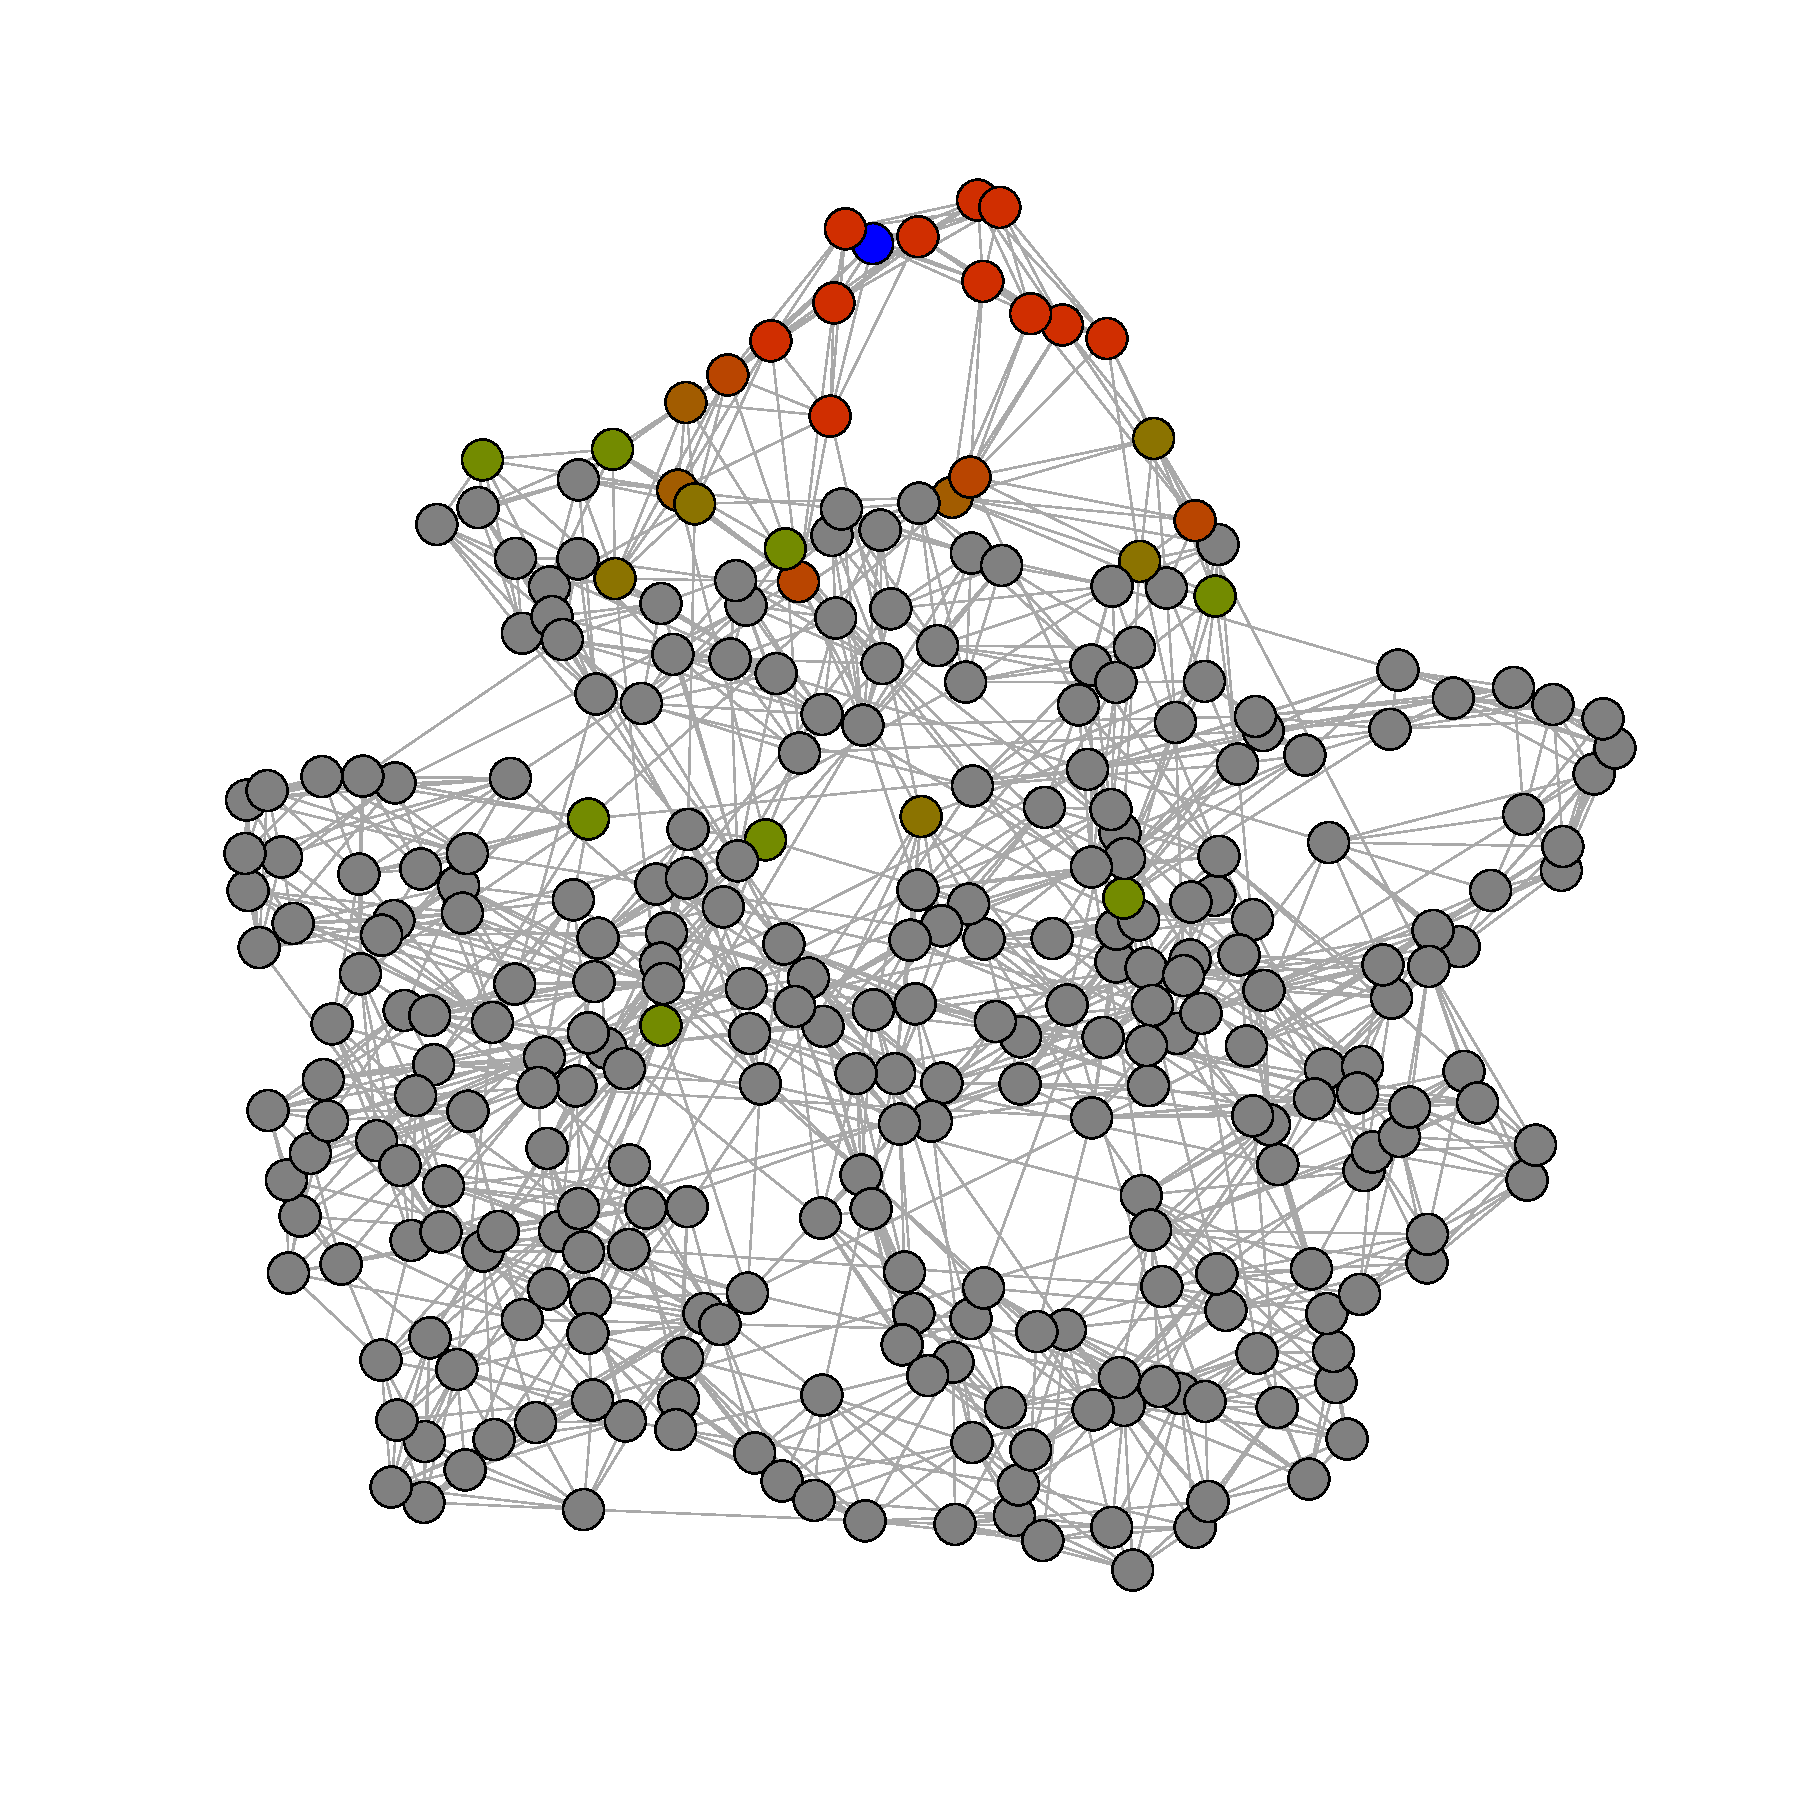
\includegraphics[width=\linewidth]{../figures/illustration_Contagion.pdf}
	\caption{Illustration of how information spreads throughout the network. The plot shows the reputation of the blue node among other members of the network. Grey nodes have never heard of the player (or have a neutral opinion), green nodes have a positive image of the blue player, whereas red nodes have a negative one. This figure illustrates that when information spreads in a contagion-based manner, closer nodes are more likely to receive the information.}
	\label{illustrate_Contagion}
\end{figure}

%-- secondary benefit: eliminating the problem of wasteful altruism
In addition to replacing the flawed concept of perfect information with a much more realistic one, this approach also solves another problem in the conventional method: Once a player has attained the highest possible image score, he has no incentive to cooperate further, because it won't benefit him. Consequently, the only rational choice is to defect (although this strategy is usually not even implemented, which means players are just downright 'wasteful' and irrational). Therefore, even an altruistically-minded person would always oscillate between the highest and second highest image score. Clearly, this is a little odd. In my methodology, this never becomes a problem. Even a player who has always cooperated will (virtually) always have someone in his immediate or at least proximate neighborhood who has not heard about his good deeds yet. Consequently there is still an incentive to be cooperative.

%-- generation & replication
With the new information dissemination mechanism in place, the simulation proceeds as following: After one round has been played out and image scores (as well as fitness scores) have been changed, 9 additional iterations are played. Then, the players 'procreate' in accordance with their evolutionary fitness: Strategies $k$ are replicated in a new network of the same size, proportional to the fitness of all players who have adopted that strategy. The more successful a specific strategy, the higher its rate of replication. Therefore the 'children' carry on the strategy of their 'parents'. Image and fitness scores are however reset to zero. One round of simulations consists of 100 of these 'generations' (each of which consists of 10 rounds, in each of which every player gets to play the donation game once). The prevalence of every strategy (indicated by how many of the players use it) is recorded at the end of each generation, so that their evolutionary viability, through their stability over time, can be assessed.

%-- topology - real world explanation
Human societies differ not just with regard to sheer size, but also in how dense they are: In a village of 500 inhabitants, the average citizen might regularly interact with 10, 50 or 100 other people. Additionally, those people may know each other at different rates as well. Furthermore, people may only interact with those who live close to them, or also have friends at the other end of the town. All of these factors could potentially affect altruistic behavior, because someone's propensity to do a good deed may depend on who will learn about it. Or, alternatively, egoistically-minded people might fare better if their fellow citizens haven't heard about their reputation yet, which could also depend on network density and the spread of information.

%-- topology
The network is randomly generated via the Watts-Strogatz model \citep{Watts1998}. This algorithm is already customary in the literature because it approximates real population structures \citep{Santos2008,Peleteiro2014}.\footnote{For the generation of a network via the Watts-Strogatz model, the R package \texttt{igraph}, version 1.2.1, is used.}\footnote{Although my argument specifically centers around the Watts-Strogatz model and its small-world property, I also experimented with two other frequently used random graph models: The Barabasi-Albert model, and the Erd\H{o}s-R\'{e}nyi model. Unsurprisingly, maintaining altruism at larger population sizes is very difficult in both cases.} The Watts-Strogatz model, often referred to as a small-world model, constructs a network as following: All nodes are placed in a ring lattice, in which each node is connected to its $l$\footnote{In the original notation style of \cite{Watts1998}, this parameter is referred to as $k$. However, since this letter already denotes the players' strategies here, I use $l$ as a substitute.} nearest neighbors. Then, each edge is rewired (i.e. one end is connected to a different node) randomly with probability $p$ (if this leads to the creation of a duplicate edge, said edge is omitted). For low values of $p$, the original ring lattice is largely preserved and the graph takes on the small-world property - high clustering (i.e. highly localized density) and small path length (i.e. no connections from one end of the network to another). One measure used to illustrate this is modularity, which measures the degree to which a graph is split into subgraphs. I illustrate this by simulating 1000 Watts-Strogatz networks, varying $p$ from $0.05$ to $1$. The results are shown in figure \ref{illustrateWS_p_modularity} -- it is evident that modularity is greater for lower levels of the rewiring probability $p$.

%-- show that p regulates 'neighborhoodness' by showing a plot with simulated random networks, p on the x-axis, and modularity on the y-axis
\begin{figure}
	\centering
	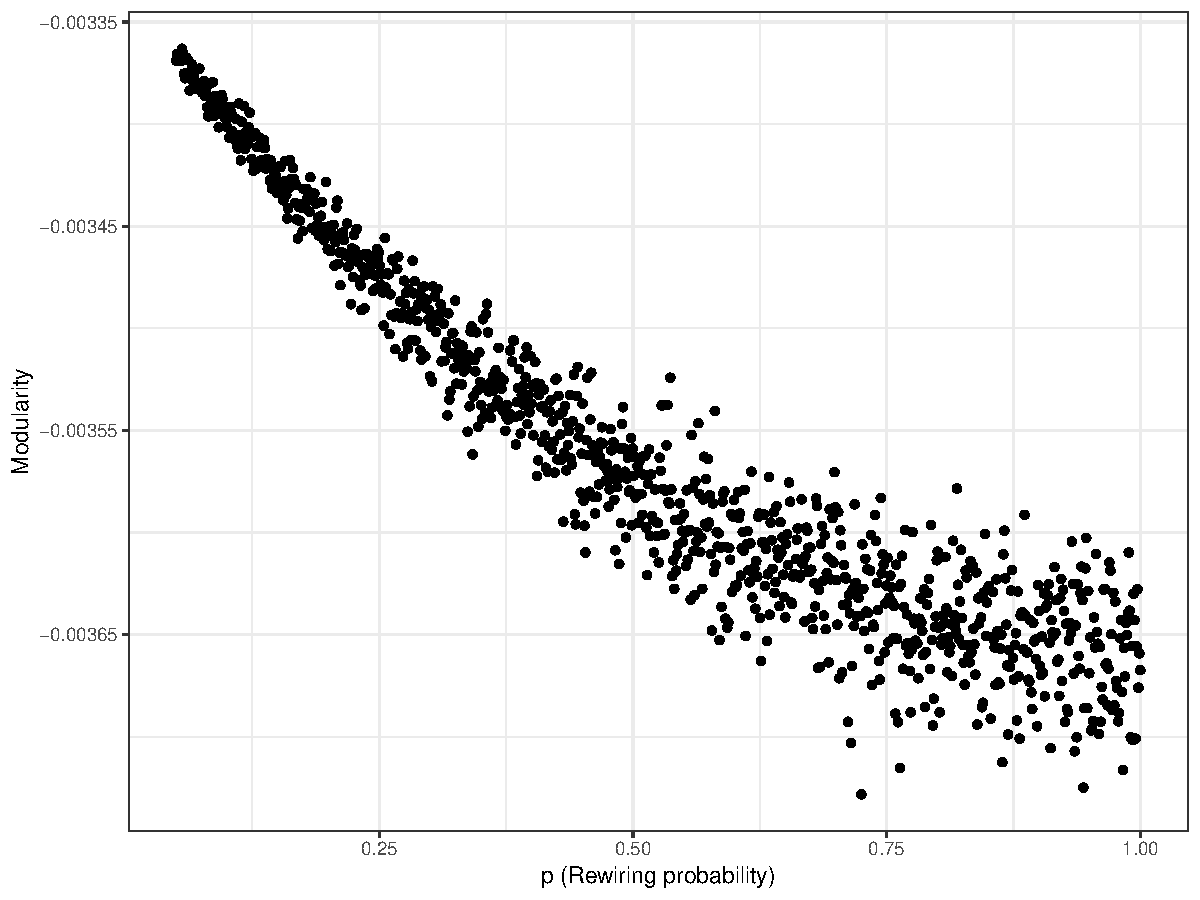
\includegraphics[width=\linewidth]{../figures/illustrateWS_p_modularity.pdf}
	\caption{1000 Watts-Strogatz networks are generated, varying $p$ from $0.05$ to $1$. Modularity measures the degree to which the network clusters into small communities. This plot demonstrates that as $p$ increases, the degree to which these neighborhoods are formed decreases.}
	\label{illustrateWS_p_modularity}
\end{figure}

As a starting point, I simulate models with parameters similar to \cite{Peleteiro2014}: A rewiring probability of $p=0.1$ and a neighborhood coefficient of $l=5$ are used. I begin with a population size of 300. Over the course of my analysis, these parameters are varied.

Figure \ref{WS_300_illustrate_p} shows examples for the Watts-Strogatz network at two different values of $p$. For $p = 0.05$, individual neighborhoods are clearly visible. By contrast, at $p = 0.3$, connections between opposite ends of the graph are more common, and local clustering is much less prevalent. The larger $p$, the more closely the Watts-Strogatz network resembles the Erd\H{o}s-R\'{e}nyi random graph, where connections are simply assigned at random. The expectation is that as $p$ increases and neighborhoods start to vanish, the conditions should become less conducive to altruistic behavior.

\begin{figure}%
	\centering
	\subfloat[Watts-Strogatz network generated with $p=0.05$.]{{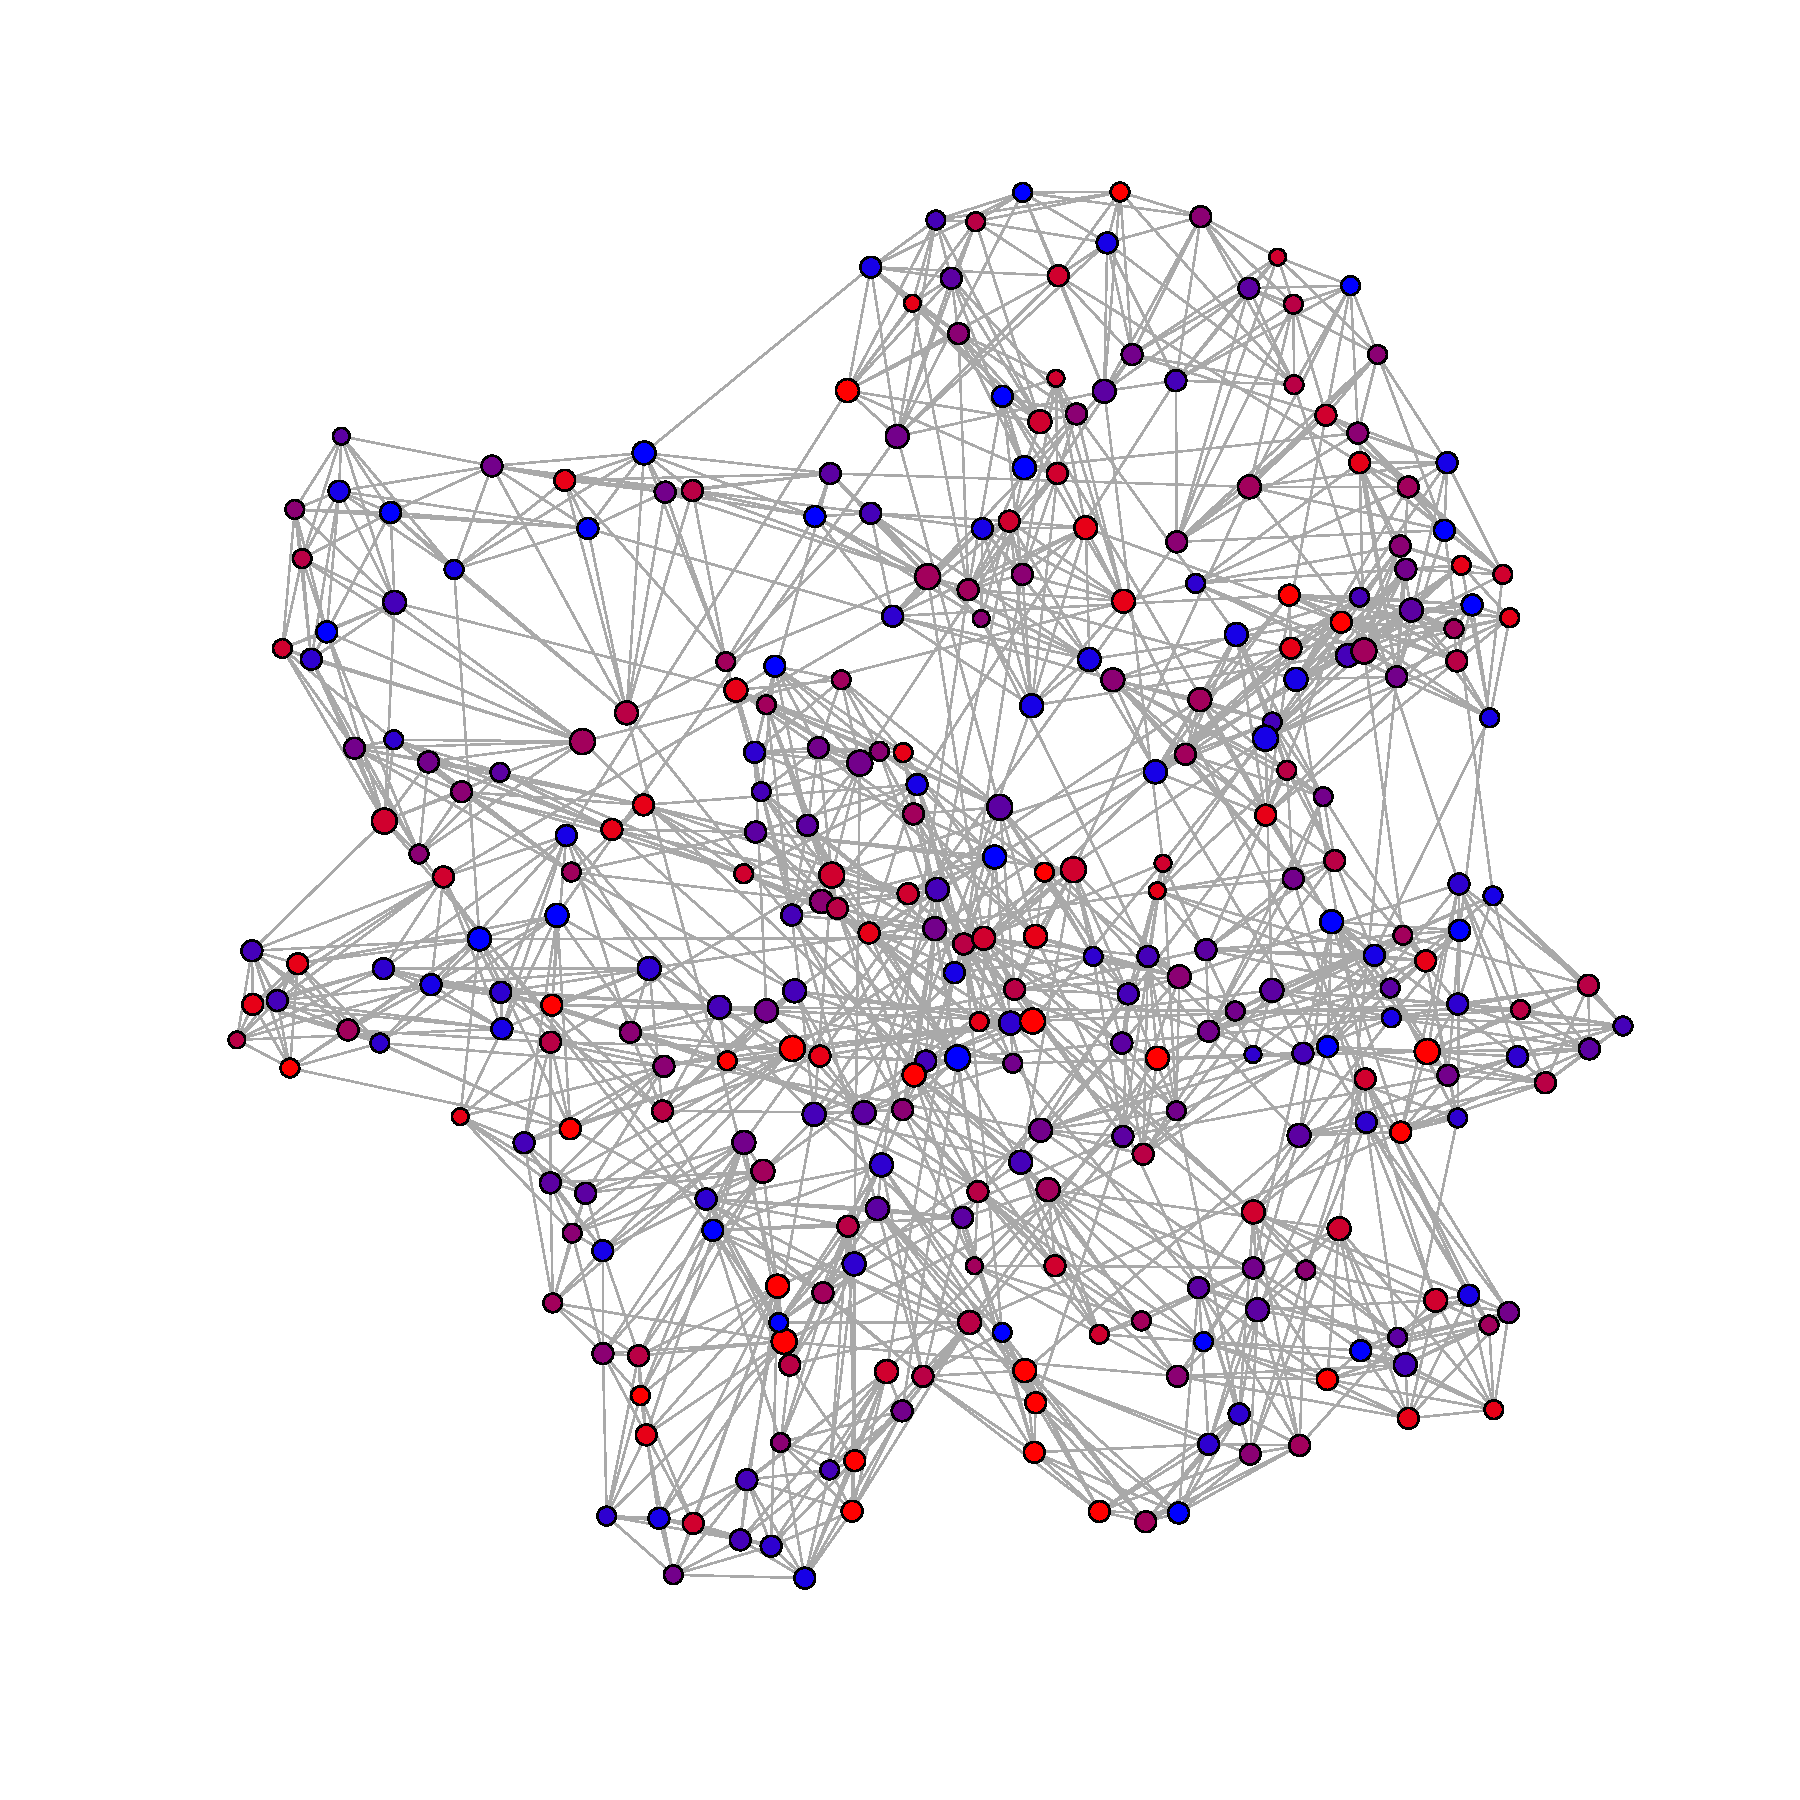
\includegraphics[width=0.46\linewidth]{../figures/illustrationWS_p005.pdf} }}%
	\qquad
	\subfloat[Watts-Strogatz network generated with $p=0.3$.]{{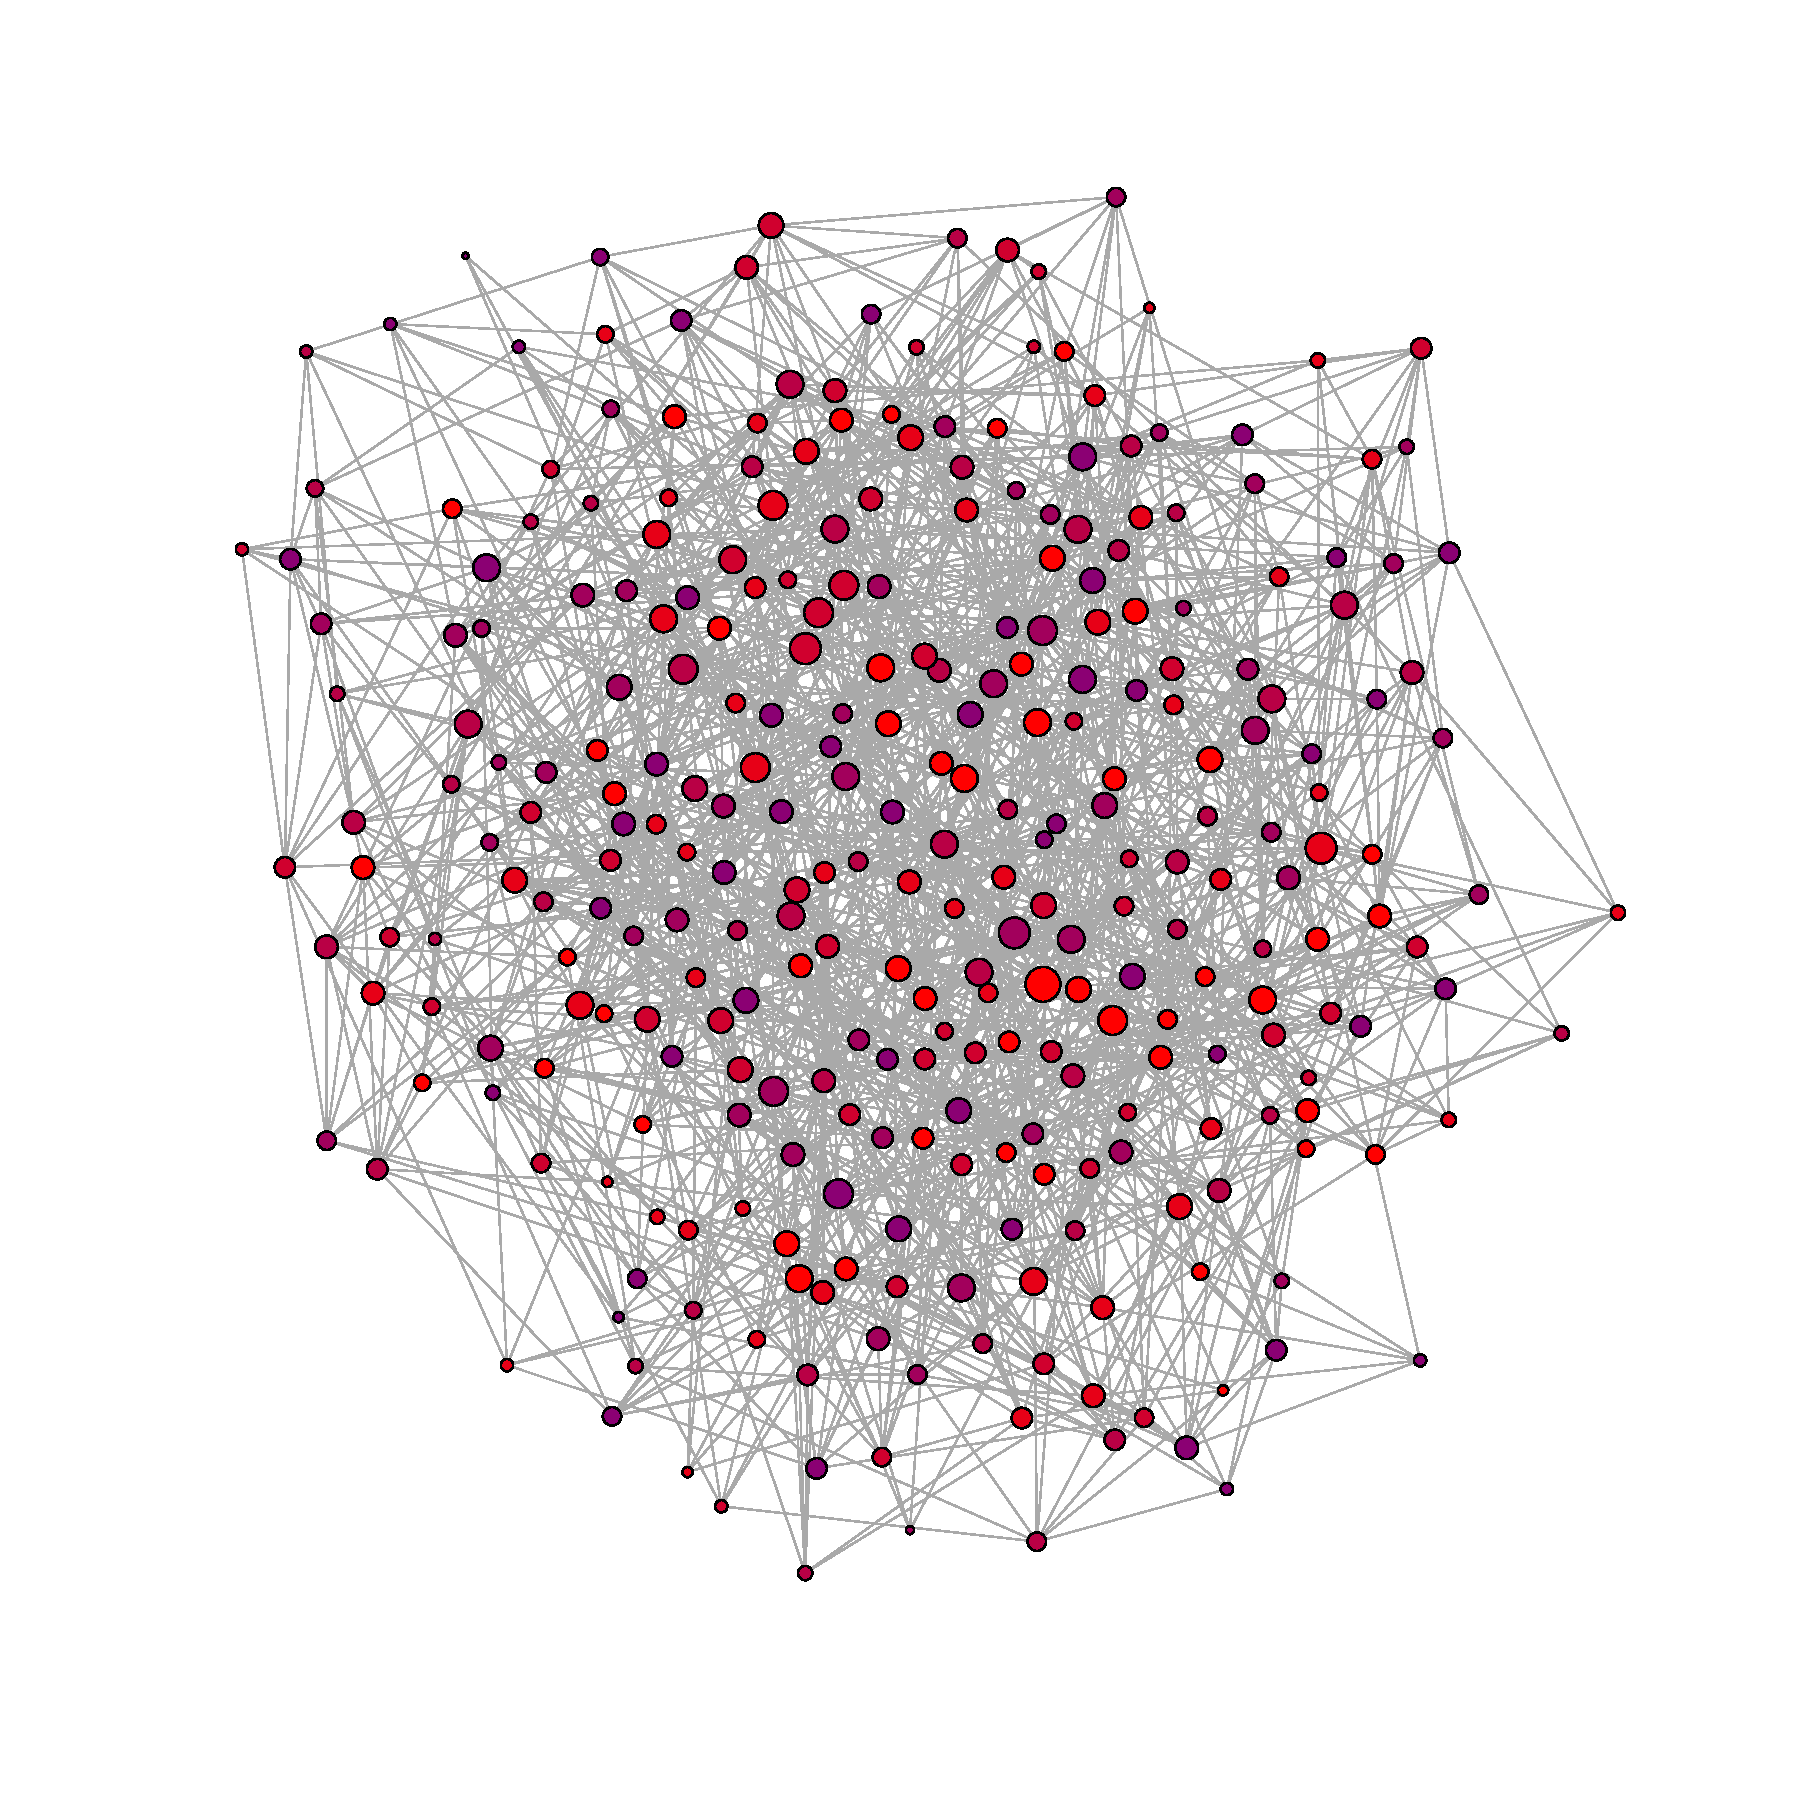
\includegraphics[width=0.46\linewidth]{../figures/illustrationWS_p03.pdf} }}%
	\caption{A comparison of the Watts-Strogatz model with  the connectivity parameter $p=0.05$ on the left and $p=0.3$ on the right. The colors denominate the strategies of the players at the end of a simulation, with blue corresponding to the most altruistic, and red to the most egoistic strategy. Larger nodes have more edges.}%
	\label{WS_300_illustrate_p}%
\end{figure}

\section*{Results: Altruism Endures in Small-World Societies}
%-- illustrate simulation
To illustrate how the simulation works, I begin by showing an example in which altruism \textit{does not} survive, and then move on to exploring conditions under which it becomes a stable strategy. Figure \ref{WS_300_p_03} provides an example for how different strategies survive over the course of 100 generations (with N=300, $p=0.2$ and $l=5$). Every point on the x-axis represents one generation, while the y-axis denotes the percentage with which a specific strategy occurs among the population. For example, at the end of the first generation, 24 players, or 8 percent of the population, are playing strategy $k=3$.

\begin{figure}
	\centering
	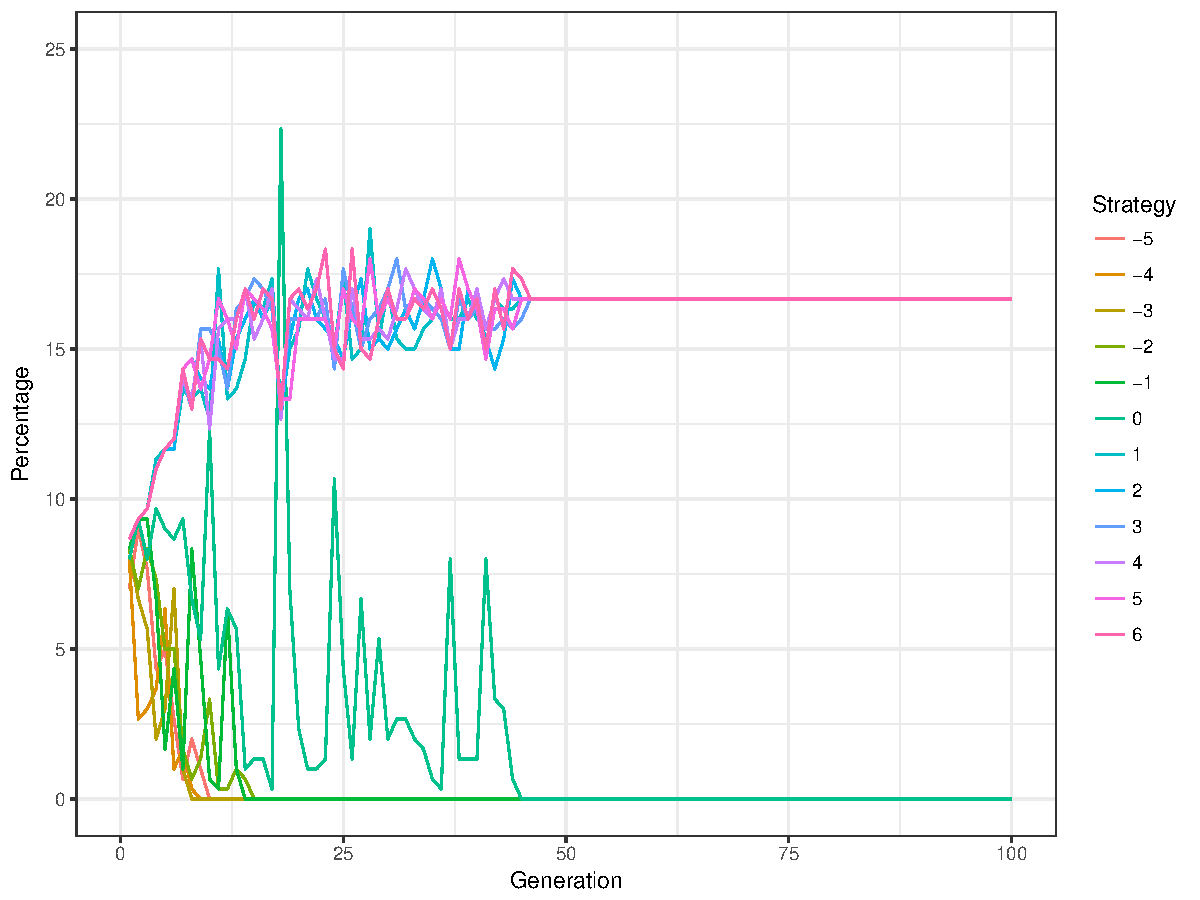
\includegraphics[width=\linewidth]{../figures/results_WS_300_p02.pdf}
	\caption{Every player in a Watts-Strogatz network generated with $p=0.2$ and $l=5$ plays the donation game once per round. After ten rounds, they replicate at a rate proportional to their relative fitness. The data points correspond to the percentage of players pursuing a particular strategy (with $k=-5$ being never defect, and $k=6$ being always defect) after one such generation.}
	\label{WS_300_p_03}
\end{figure}

Since strategies are randomly distributed at the beginning of the simulation, it takes a while until they begin to sort themselves out. However, it becomes evident quite quickly that the strategies associated with greater egoism (i.e. $k>0$) are more stable. By contrast, the altruistic strategies $k<=0$ fluctuate wildly, and after about 20 generations, begin to die out one after another. There are a handful of cases in which the mildly altruistic, or in this case, the neutral strategy ($k=0$ at generation 18) actually surpass the egoistic strategies for a short while. However, rather than a sustainable trend, this is more of a 'last hurrah', after which the strategy quickly flickers out again. This demonstrates that no mutant is able to invade the set of evolutionarily stable strategies \citep{hamilton1964_2}.

%The most altruistic strategy that manages to survive at all is $k=0$, i.e. the strategy that strictly discriminates between altruistic and egoistic players. Importantly, this strategy never reaches a constant rate of survival, but instead fluctuates throughout all generations. This is not a random result that occurs only in this particular run of simulations, but instead happens repeatedly, under a wide range of different parameters. This indicates that there might be something special about this strategy, to be explored in future research.

Finally, the strategies $k>0$ quickly become dominant and stay that way for the rest of the simulation. However, among these strategies, no single one emerges as preeminent. Instead, they fluctuate around, and eventually converge to the same value. This behavior is also present in my other simulations and stems from the degree of randomness introduced by the information contagion mechanism.

\begin{figure}
    \centering
    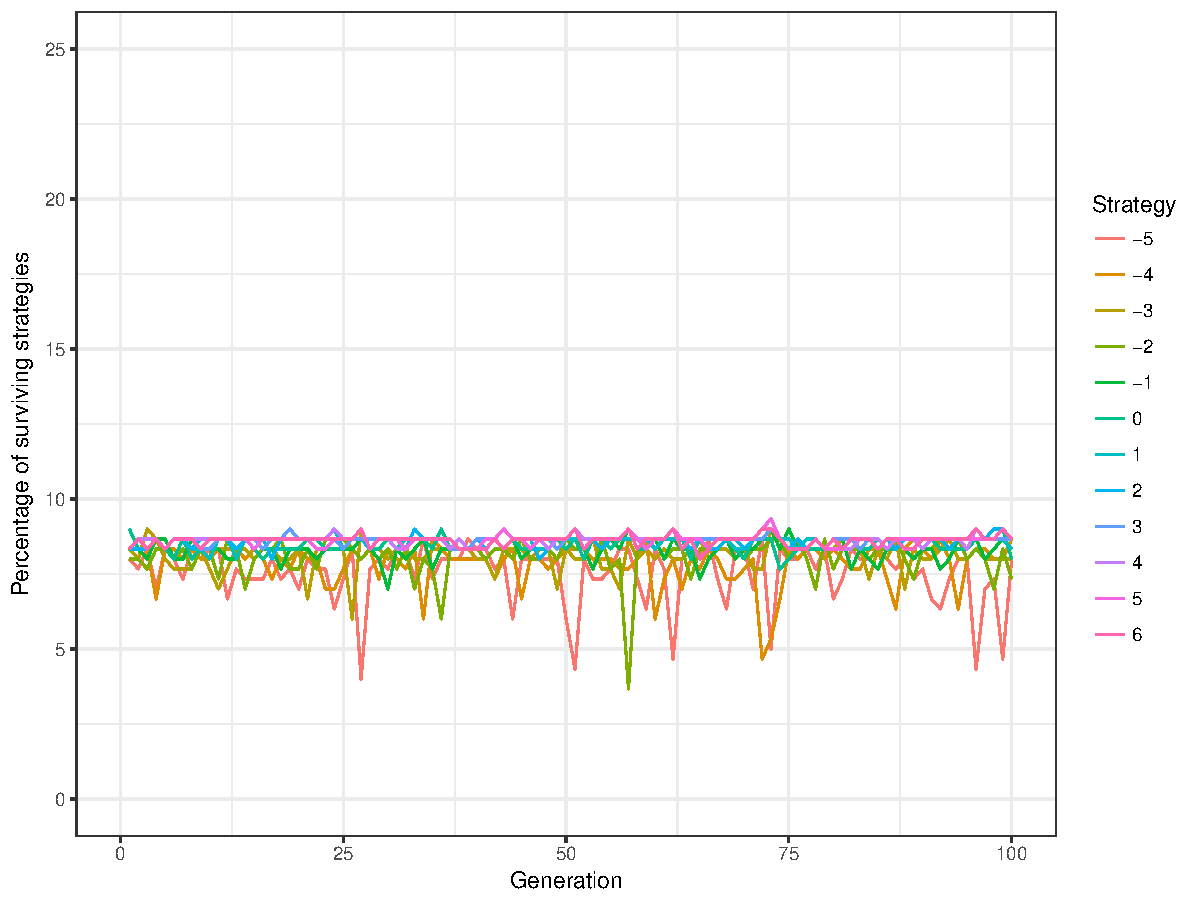
\includegraphics[width=\linewidth]{../figures/results_WS_300_default.pdf}
    \caption{Every player in a Watts-Strogatz network generated with $p=0.1$ and $l=5$ plays the donation game once per round. After ten rounds, they replicate at a rate proportional to their relative fitness. The data points correspond to the percentage of players pursuing a particular strategy (with $k=-5$ being never defect, and $k=6$ being always defect) after one such generation.}
    \label{WS_300_default}
\end{figure}

%-- altruism survives if p is low
Figure \ref{WS_300_default} three shows the results of a similar simulation, this time using a value of $p=0.1$ instead of $p=0.3$. The differences are quite striking: Convergence occurs immediately, all strategies fluctuate only slightly, and around the same value. None of them are dominant in any way, $k=-5$ (never defect) occurs just as much as $k=6$ (always defect). Comparing these results to the ones obtained from the Barab\'{a}si-Albert algorithm shows that network topology can make a huge difference as far as the evolutionary stability of altruism is concerned.

\begin{figure}
    \centering
    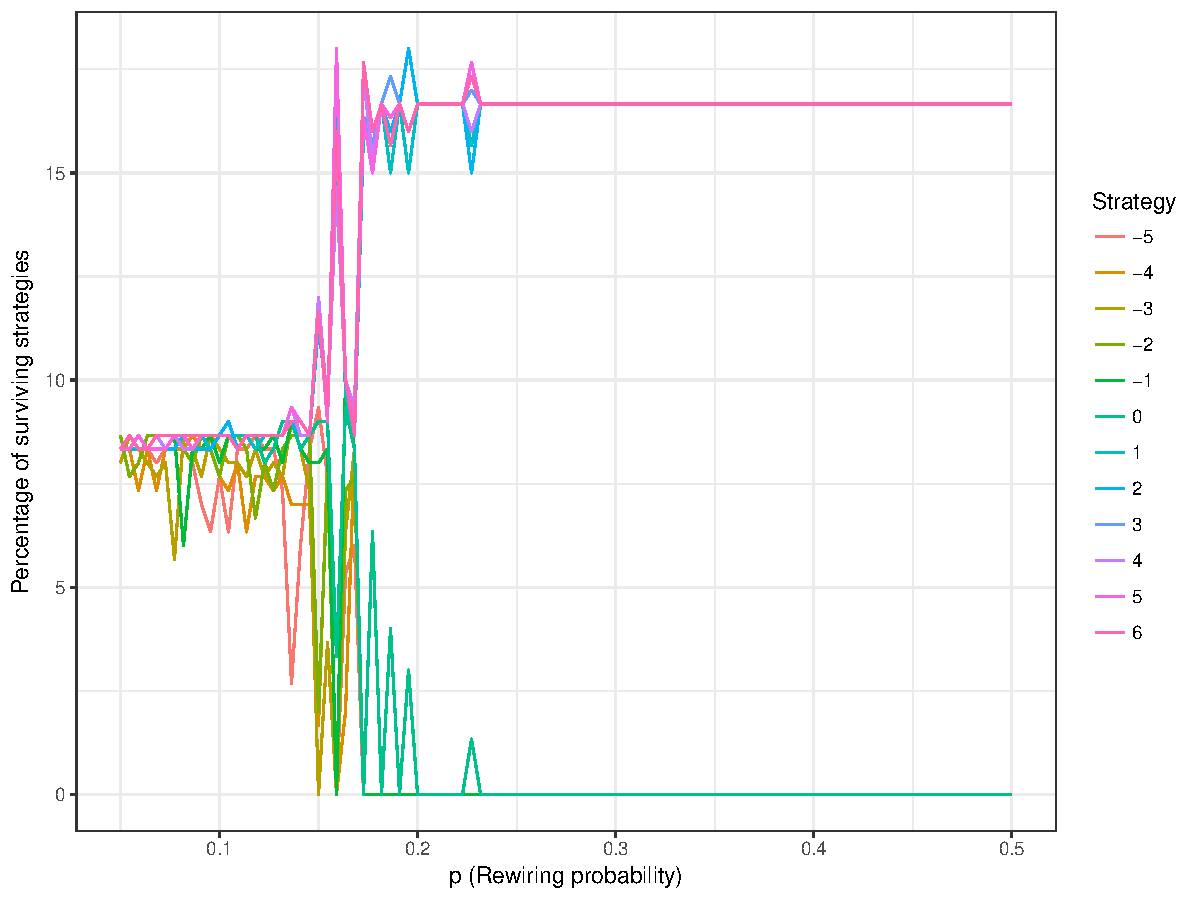
\includegraphics[width=\linewidth]{../figures/results_WS_300_p_100sims.pdf}
    \caption{The simulation is conducted 100 times, varying the connectivity parameter $p$ in a Watts-Strogatz network. The data points correspond to the percentage of players pursuing a particular strategy (with $k=-5$ being never defect, and $k=6$ being always defect) after the 100th generation in each simulation.}
    \label{WS_300_p_100sims}
\end{figure}

%-- simulate different values of p
To further elucidate the impact of network topology, and the connectivity parameter specifically, figure \ref{WS_300_p_100sims} presents the results of 100 simulations using the Watts-Strogatz algorithm, where the connectivity parameter $p$ is varied. Importantly, this plot is different from  figures \ref{WS_300_p_03} and \ref{WS_300_default}: Before, the values described the results after each generation, from only one simulation. Figure \ref{WS_300_p_100sims} on the other hand is the result of 100 individual simulations, each with a different value for $p$. Here, the values on the y-axis denominate the distribution of strategies after the last generation of each of these simulations (i.e. when they have converged). At comparatively low levels of connectivity (however, it should be noted that even a value of 0.1, as used above, already leads to a fairly dense network) the results mirror figure \ref{WS_300_default}, but once it gets higher, the altruistic strategies start to fluctuate. Finally, at 0.3, this fluctuation becomes much stronger until one after another, these strategies die out. For high connectivity levels, the strategy distribution is very similar to what it would be under the Barab\'{a}si-Albert algorithm.\footnote{The results for the other network parameter $l$ can be found in figure 7, 8 and 9 in the appendix. The neighborhood coefficient in does not appear to affect altruism.}

\begin{figure}
    \centering
    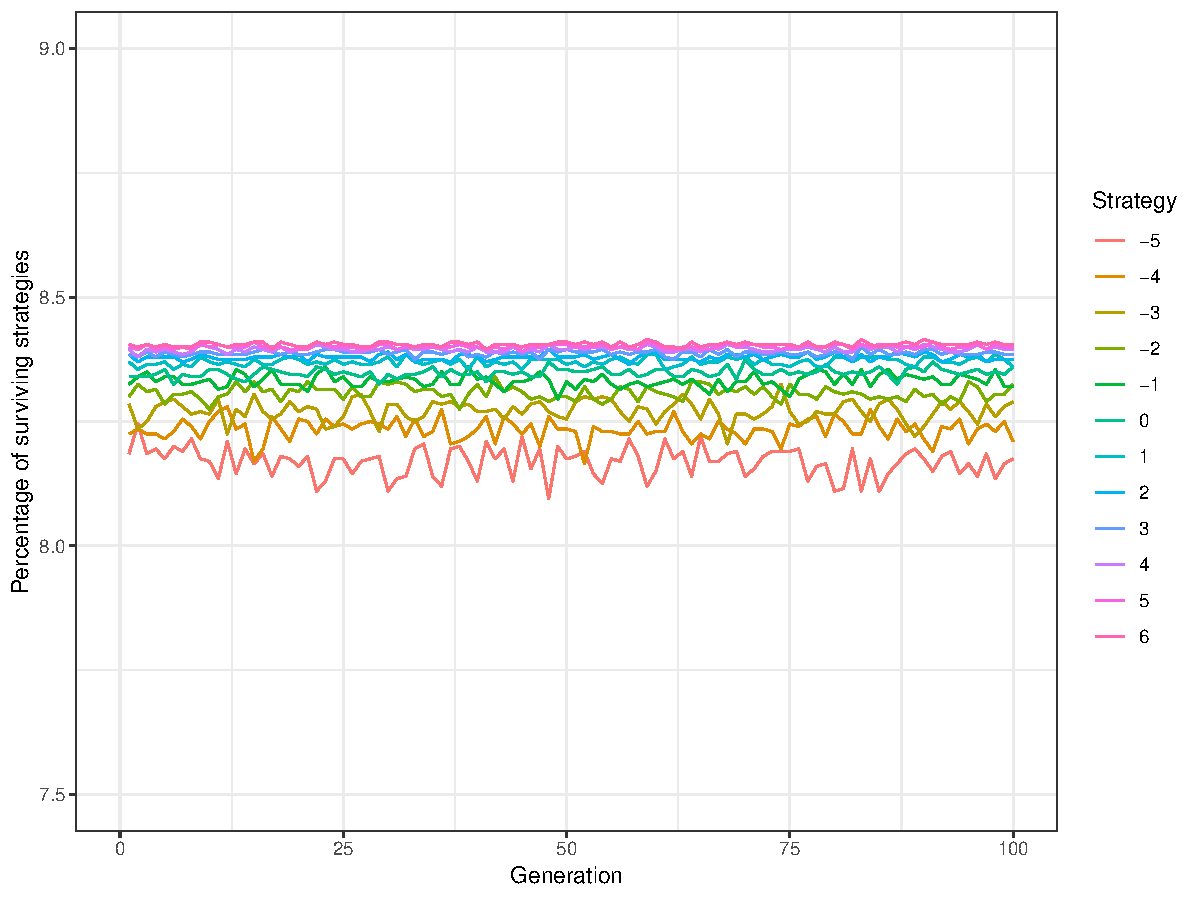
\includegraphics[width=\linewidth]{../figures/results_WS_20000_p005.pdf}
    \caption{Every player in a Watts-Strogatz network with a population of 20,000 plays the donation game once per round. After ten rounds, they replicate at a rate proportional to their relative fitness. The data points correspond to the percentage of players pursuing a particular strategy (with $k=-5$ being never defect, and $k=6$ being always defect) after one such generation.}
    \label{WS_20000_default}
\end{figure}

%-- altruism survives at N=20000 if p is low
Having established that the degree to which a Watts-Strogatz network forms local neighborhoods, modulated by the rewiring probability $p$, affects the degree of altruism that is possible in the network, I can now put this knowledge to use in simulating a large random network under conditions amenable to altruism. Figure \ref{WS_20000_default} shows the results of a simulation with the Watts-Strogatz model, using the same parameters as for figure \ref{WS_300_default} ($p=0.1$ and $l=5$), but with a population of 20,000. In keeping with my hypothesis, altruistic behavior at such a large population size is now feasible. That being said, while altruistic strategies are viable and stable, pure egoism is the most successful. This result stands in contrast to smaller population sizes, where all strategies were either equally successful, or died out entirely. However, it is very important to note that the differences are small, as even $k=-5$ still makes up around 8.2 percent of the population (as opposed to roughly 8.4 percent for $k=6$). The differentiation between degrees of egoism (i.e. $k<0$) does not occur anywhere else and appears to be entirely dependent on population size.

\section*{Discussion}
What can we learn from all this? Clearly, network topology matters a great deal. Networks which cluster into small neighborhoods, where everyone knows everyone else and interacts with them on a regular basis are more conducive to altruism. Essentially, these neighborhoods form smaller sub-networks, and as the literature has shown, smaller populations are more likely to produce selfless behavior. By contrast, when connections exist evenly throughout the graph, altruistic behavior becomes less feasible. This is because in a network with heavy clustering, a node's neighbor is more likely to be connected to another neighbor of the original node.

This is where my contagion-based information dissemination mechanism comes in. In a conventional network with perfect information, clustering is not as important, as all of a node's immediate neighbors will always learn about its reputation. But if information about a player spreads on the basis of contagion, its neighbors it did not interact with that turn will be much more likely to find out in a network with high modularity. By contrast, when clustering is low, it does not matter as much if they annoy some of their neighbors through non-cooperative behavior, because there are still enough other players around who have not heard about their exploitative deeds yet.

Once the necessary network structure is in place, scaling up the population to $N>1000$ without making altruism non-viable becomes less of a problem than it has been in prior research. As long as the rewiring probability is low, the network consists of small neighborhoods, and since the players predominantly interact with other players within their neighborhoods rather than across the network, repeat interactions are common, and information spreads quickly among their neighbors. Consequently, altruistic strategies can survive.

%Algorithms used by other researchers tend to converge to one single strategy, for example to $k-3$ \citep{Peleteiro2014}. This is due to the fact that with perfect information, the stochastic component of these models is much smaller. These mechanisms are very 'all-or-nothing', so when the population size is increased (which verifiably decreases altruism), the pendulum swings to 'nothing' all too easily.

When comparing the effects of varying network topology and size, it becomes clear that while size matters, topology turns out to be another powerful determinant of altruism. This is an important finding, because previous research has not been conclusive in this matter: \cite{Santos2008} and \cite{Peleteiro2014} compare the Barabasi-Albert and Watts-Strogatz models, but their simulations don't actually fully exploit the fairly big differences between these two types of networks. Furthermore, they do not test for the effect of changing the network parameters. My model is more sensitive to changes in network topology and thus reveals the full repercussions of variation in it.

%Another interesting finding is the fact that many times, the strategy $k=0$ is the most altruistic one to survive. What makes this strategy so special? The answer to that question is simple: it discriminates maximally. For image scores $s_j \in [-5,-1]$ a player who chooses $k_i=0$ defects, for $s_j \in [0,5]$ he cooperates. Ergo, among all the altruistic strategies, it is the least likely to be 'suckered'. It is the 'wary cooperator' \citep{Hibbing2004}.

%How does all of this translate to the real world? The Barab\'{a}si-Albert model has often been likened to vertical hierarchies, because it contains a small number of extremely well-connected individuals, whereas everyone else exists at the fringes of the network. By contrast, the Watts-Strogatz algorithm produces a set of much more evenly distributed edges. This resonates with the arguments made in \cite{Fowler2005a}, who situate egalitarianism as a major driving force behind the emergence and continued existence of altruism.

%facebook
%My findings indicate that networks in which superficial connections are formed with casual acquaintances

%The adage ''do good and talk about it'' actually makes sense here.


%It is also worth pointing out that while altruism can easily die out if the condition aren't right, the opposite is not true. Throughout all of my simulations, egoistic strategies (i.e. $k>0$) always survived. Defecting carries much less risk with it, and networks in which altruism does exist also make it easier for exploitative strategies.

In conclusion, my research contributes to the extant literature by improving the widely-used image score mechanism, introducing an element of imperfect information. Furthermore, it demonstrates that a great deal of variation in altruism can be explained through network topology. Finally, I manage to show how selflessness can exist even in larger societies. With that said, I will let the bard \citep{Shakespeare} have the last word: ''How far that little candle throws his beams! So shines a good deed in a naughty world.''

\newpage

\bibliographystyle{apsr}
\bibliography{Markus_Altruism_Bib}

\newpage
\section*{Supplemental Information}
The following pseudo-code provides a simplified overview of the simulation.\footnote{The full replication code is located at: \url{https://github.com/markusneumann/altruism_simulation}} Algorithm \ref{Algorithm1} details the overarching framework of the simulation. First, a Watts-Strogatz network is created according to a set of parameters: population size $N$, rewiring probability $p$ and neighborhood coefficient $l$. If any of the players are isolates (i.e. they have no connections), the network is re-generated until all players are properly connected. Then, 100 generations of the population 'live their lives'. Each of these consist of 10 rounds. In every one of these rounds, the donation game, specified in algorithm \ref{Algorithm2}, is played. After the completion of this stage, information about the players' actions is spread through the population according to algorithm \ref{Algorithm4}. Once 10 such rounds have concluded, the number of players using each strategy is recorded. For example, after 15 generations in a Watts-Strogatz network, the strategy $k=0$ is used by 25 players. Ergo, 8.3 percent ($25/300=0.083$) is the y-value for $k=0$ at $x=15$ in figure \ref{WS_300_default}. Finally, the players replicate, as denoted in algorithm \ref{Algorithm4}.

\begin{algorithm}
	\caption{Simulation}
	\label{Algorithm1}
	\begin{algorithmic}[1]
		\Function{Simulation}{}
		\State $\text{Specify network parameters}$
		\State $\text{Create network}$
		\For{\text{g in 100 generations}}
		\For{\text{r in 10 rounds}}
		\State $DonationGame$
		\State $InformationDissemination$
		\EndFor
		\State $\text{(Record results)}$
		\State $Replication$
		\EndFor
		\EndFunction
	\end{algorithmic}
\end{algorithm}

Algorithm \ref{Algorithm2} describes the donation game. Every member of the population gets to be player 1 once. The first thing he does is to determine who his neighbors (i.e. nodes to which he is connected through an edge) are. Of these, one is randomly selected to be player 2. Then the game begins: Player 1 determines whether his own strategy $k_i$ is smaller or equal to his impression of his ``opponent's'' image score $s_{ij}$. If it is, a donation takes place and player 1's fitness is decreased by $1$, while player 2's fitness is increased by $2$. Furthermore, the variable $s_i$, which denotes whether or not player 1 has helped, is set to $1$. If $k_i>s_{ij}$, no donation occurs, and $s_i$ is set to $-1$. Ergo, as in the classical form of the donation game without the spread of information, $s_i$ is an objective measure of what player 1 has done. However, it is only valid for the current round.

\begin{algorithm}
	\caption{Donation game}
	\label{Algorithm2}
	\begin{algorithmic}
		\Function{DonationGame}{}
		\For{\text{N times}}
		\State $i_{n}.FindNeighbors(j\in[N];j\neq i)$
		\If {$k_i\leq s_{ij}$}
		\State $f_i \gets f_i-1$
		\State $f_j \gets f_j+2$
		\State $s_{i} \gets 1$
		\Else
		\State $s_{i} \gets -1$
		\EndIf
		\EndFor
		\EndFunction
	\end{algorithmic}
\end{algorithm}

Algorithm \ref{Algorithm3} determines if and how other players actually learn about $s_i$. For every donation game played in algorithm \ref{Algorithm2}, information is disseminated through the network as following: Since player 2 was directly involved, he always learns about the donation. His impression of player 1, $s_{ij}$, is updated by adding $s_i$ to it. Then his neighbors are determined. For each neighbor, a Bernoulli trial with a 50 percent chance of success is conducted. Every neighbor $c$ for whom this trial is successful, learns about the donation and updates his image of player 1 ($s_{ci}$). Then all players $h$ repeat this process and spread the information to their neighbors $d$ with a 25 percent probability for each, who do the same to their neighbors $e$ with a 12.5 percent chance.

\begin{algorithm}
	\caption{Information dissemination}
	\label{Algorithm3}
	\begin{algorithmic}
		\Function{InformationDissemination}{}
		\For{\text{every donation game}}
		\State $s_{ji} \gets s_{ji}+s_{i}$
		\State $j.FindNeighbors(c\in[N];c\neq i,j)$
		\For{\text{every neighbor c}}
		\State $c_z \gets \text{Bernoulli trial(prob=0.5)}$
		\If {$c_z=1$}
		\State $s_{ci} \gets s_{ci}+s_{i}$
		\State $c.FindNeighbors(d\in[N];d\neq i,j,c)$
		\For{\text{every neighbor d}}
		\State $d_z \gets \text{Bernoulli trial(prob=0.25)}$
		\If {$d_z=1$}
		\State $s_{di} \gets s_{di}+s_{i}$
		\State $d.FindNeighbors(e\in[N];e\neq i,j,c,d)$
		\For{\text{every neighbor e}}
		\State $e_z \gets \text{Bernoulli trial(prob=0.125)}$
		\If {$e_z=1$}
		\State $s_{ei} \gets s_{ei}+s_{i}$
		\EndIf
		\EndFor
		\EndIf
		\EndFor
		\EndIf
		\EndFor
		\EndFor
		\EndFunction
	\end{algorithmic}
\end{algorithm}

At the end of a generation, all players 'die' and pass on their strategies to their 'children'. This process is outlined in algorithm \ref{Algorithm4}. Replication is modeled by calculating the relative success of each strategy compared to all others. Then, a new network is created in which the strategies are distributed accordingly. This is done as following: For each strategy $k$, I determine the average fitness of all players who follow it. The result is a 12-element vector, containing one mean value for each strategy. In order to avoid erratic results due to outliers, I apply the inverse logit function. Then, each value is divided by the sum of the vector, to calculate the relative success of each strategy. This value is multiplied by the population size $N$, for the number of players who will use that strategy in the next generation. This value is then rounded to the nearest whole number.

If the sum of the resulting values does not equal the population size (due to rounding error), I add or subtract randomly selected strategies until they do. This can lead to the reintroduction of strategies that have already died out (although as noted above, they never survive long). Thus, I explicitly test for the assumption that no mutant can successfully invade an evolutionarily stable strategy distribution \citep{hamilton1964_2}. This concludes the final stage of a generation, the replication.

\begin{algorithm}
\caption{Replication}
\label{Algorithm4}
	\begin{algorithmic}
		\Function{Replication}{}
		\For{\text{every strategy k}}
		\State $r_k=\text{average fitness of all players following strategy k}$
		\State $r_k=\text{inverse logit}(r_k)$
		\EndFor
		\For{\text{every strategy k}}
		\State $r_k=round((r_{k}/sum(r))*N)$
		\EndFor
		%\State $r=r_{-5},r_{-4},...,r_{6}$
		\While {$sum(r)<N$}
		\State $\text{introduce random strategy}$
		\EndWhile
		\While {$sum(r)>N$}
		\State $\text{remove random strategy}$
		\EndWhile
		\State $\text{create new network}$
		\State $\text{assign strategies according to r}$
		\EndFunction
	\end{algorithmic}
\end{algorithm}

\begin{figure}
    \centering
    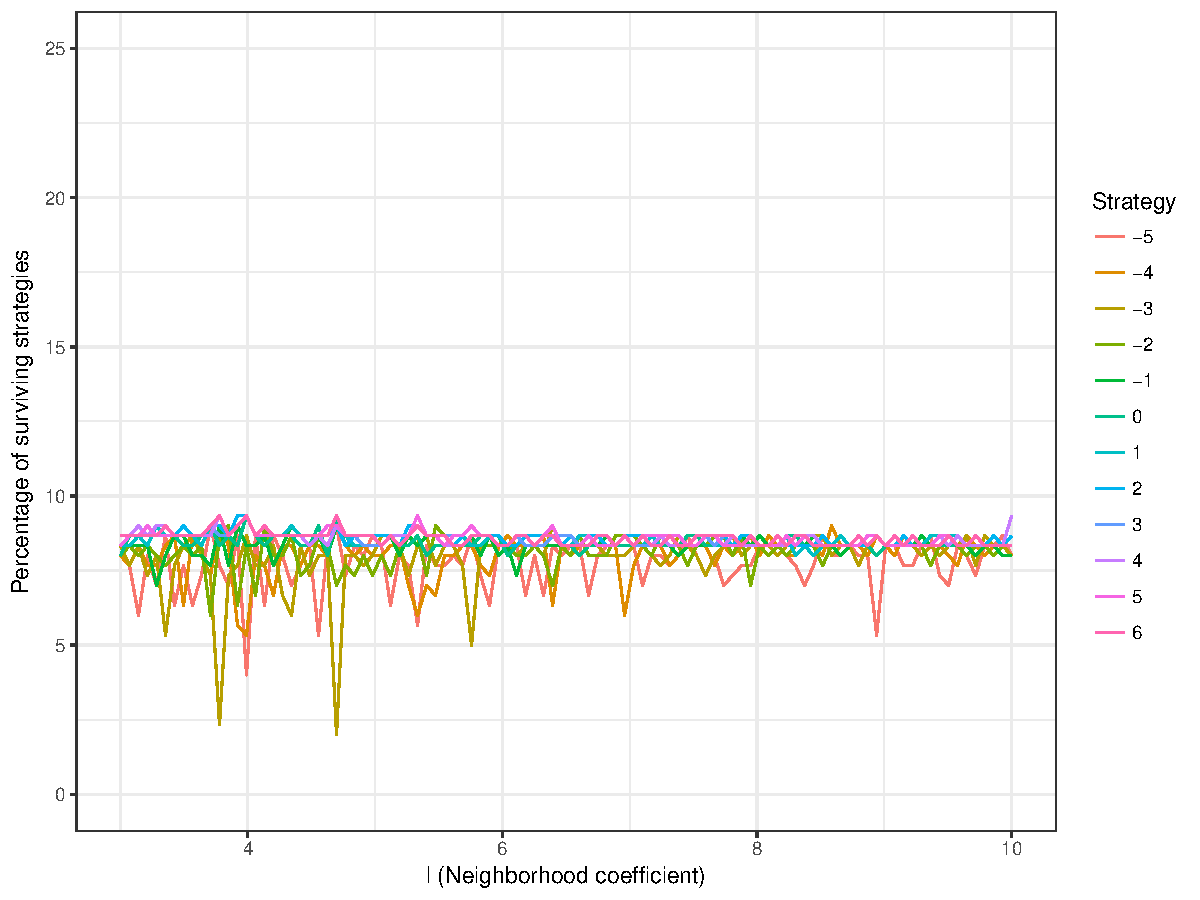
\includegraphics[width=\linewidth]{../figures/results_WS_300_nei_100sims.pdf}
    \caption{The simulation is conducted 100 times, varying the neighborhood coefficient $l$ in a Watts-Strogatz network. The data points correspond to the percentage of players pursuing a particular strategy (with $k=-5$ being never defect, and $k=6$ being always defect) after the 100th generation in each simulation.}
    \label{WS_300_l_100sims}
\end{figure}

\end{document}

%%%%%%%%%%%%%%%%%%%%%%%%%%%%%%%%%%%%%%%%%%%%%%%%%%%%%%%%%%%%%%%%%%%%%%
%% The end.
%%%%%%%%%%%%%%%%%%%%%%%%%%%%%%%%%%%%%%%%%%%%%%%%%%%%%%%%%%%%%%%%%%%%%%
